\documentclass[1p]{elsarticle_modified}
%\bibliographystyle{elsarticle-num}

%\usepackage[colorlinks]{hyperref}
%\usepackage{abbrmath_seonhwa} %\Abb, \Ascr, \Acal ,\Abf, \Afrak
\usepackage{amsfonts}
\usepackage{amssymb}
\usepackage{amsmath}
\usepackage{amsthm}
\usepackage{scalefnt}
\usepackage{amsbsy}
\usepackage{kotex}
\usepackage{caption}
\usepackage{subfig}
\usepackage{color}
\usepackage{graphicx}
\usepackage{xcolor} %% white, black, red, green, blue, cyan, magenta, yellow
\usepackage{float}
\usepackage{setspace}
\usepackage{hyperref}

\usepackage{tikz}
\usetikzlibrary{arrows}

\usepackage{multirow}
\usepackage{array} % fixed length table
\usepackage{hhline}

%%%%%%%%%%%%%%%%%%%%%
\makeatletter
\renewcommand*\env@matrix[1][\arraystretch]{%
	\edef\arraystretch{#1}%
	\hskip -\arraycolsep
	\let\@ifnextchar\new@ifnextchar
	\array{*\c@MaxMatrixCols c}}
\makeatother %https://tex.stackexchange.com/questions/14071/how-can-i-increase-the-line-spacing-in-a-matrix
%%%%%%%%%%%%%%%

\usepackage[normalem]{ulem}

\newcommand{\msout}[1]{\ifmmode\text{\sout{\ensuremath{#1}}}\else\sout{#1}\fi}
%SOURCE: \msout is \stkout macro in https://tex.stackexchange.com/questions/20609/strikeout-in-math-mode

\newcommand{\cancel}[1]{
	\ifmmode
	{\color{red}\msout{#1}}
	\else
	{\color{red}\sout{#1}}
	\fi
}

\newcommand{\add}[1]{
	{\color{blue}\uwave{#1}}
}

\newcommand{\replace}[2]{
	\ifmmode
	{\color{red}\msout{#1}}{\color{blue}\uwave{#2}}
	\else
	{\color{red}\sout{#1}}{\color{blue}\uwave{#2}}
	\fi
}

\newcommand{\Sol}{\mathcal{S}} %segment
\newcommand{\D}{D} %diagram
\newcommand{\A}{\mathcal{A}} %arc


%%%%%%%%%%%%%%%%%%%%%%%%%%%%%5 test

\def\sl{\operatorname{\textup{SL}}(2,\Cbb)}
\def\psl{\operatorname{\textup{PSL}}(2,\Cbb)}
\def\quan{\mkern 1mu \triangleright \mkern 1mu}

\theoremstyle{definition}
\newtheorem{thm}{Theorem}[section]
\newtheorem{prop}[thm]{Proposition}
\newtheorem{lem}[thm]{Lemma}
\newtheorem{ques}[thm]{Question}
\newtheorem{cor}[thm]{Corollary}
\newtheorem{defn}[thm]{Definition}
\newtheorem{exam}[thm]{Example}
\newtheorem{rmk}[thm]{Remark}
\newtheorem{alg}[thm]{Algorithm}

\newcommand{\I}{\sqrt{-1}}
\begin{document}

%\begin{frontmatter}
%
%\title{Boundary parabolic representations of knots up to 8 crossings}
%
%%% Group authors per affiliation:
%\author{Yunhi Cho} 
%\address{Department of Mathematics, University of Seoul, Seoul, Korea}
%\ead{yhcho@uos.ac.kr}
%
%
%\author{Seonhwa Kim} %\fnref{s_kim}}
%\address{Center for Geometry and Physics, Institute for Basic Science, Pohang, 37673, Korea}
%\ead{ryeona17@ibs.re.kr}
%
%\author{Hyuk Kim}
%\address{Department of Mathematical Sciences, Seoul National University, Seoul 08826, Korea}
%\ead{hyukkim@snu.ac.kr}
%
%\author{Seokbeom Yoon}
%\address{Department of Mathematical Sciences, Seoul National University, Seoul, 08826,  Korea}
%\ead{sbyoon15@snu.ac.kr}
%
%\begin{abstract}
%We find all boundary parabolic representation of knots up to 8 crossings.
%
%\end{abstract}
%\begin{keyword}
%    \MSC[2010] 57M25 
%\end{keyword}
%
%\end{frontmatter}

%\linenumbers
%\tableofcontents
%
\newcommand\colored[1]{\textcolor{white}{\rule[-0.35ex]{0.8em}{1.4ex}}\kern-0.8em\color{red} #1}%
%\newcommand\colored[1]{\textcolor{white}{ #1}\kern-2.17ex	\textcolor{white}{ #1}\kern-1.81ex	\textcolor{white}{ #1}\kern-2.15ex\color{red}#1	}

{\Large $\underline{12a_{0433}~(K12a_{0433})}$}

\setlength{\tabcolsep}{10pt}
\renewcommand{\arraystretch}{1.6}
\vspace{1cm}\begin{tabular}{m{100pt}>{\centering\arraybackslash}m{274pt}}
\multirow{5}{120pt}{
	\centering
	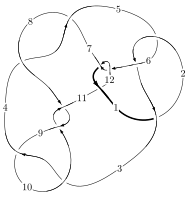
\includegraphics[width=112pt]{../../../GIT/diagram.site/Diagrams/png/1234_12a_0433.png}\\
\ \ \ A knot diagram\footnotemark}&
\allowdisplaybreaks
\textbf{Linearized knot diagam} \\
\cline{2-2}
 &
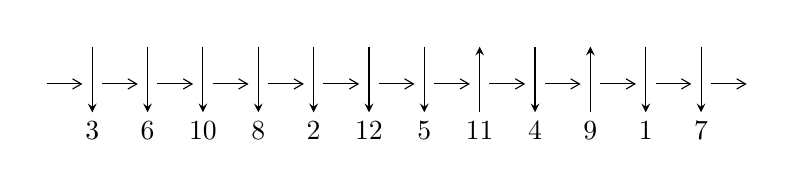
\begin{tikzpicture}[x=20pt, y=17pt]
	% nodes
	\node (C0) at (0, 0) {};
	\node (C1) at (1, 0) {};
	\node (C1U) at (1, +1) {};
	\node (C1D) at (1, -1) {3};

	\node (C2) at (2, 0) {};
	\node (C2U) at (2, +1) {};
	\node (C2D) at (2, -1) {6};

	\node (C3) at (3, 0) {};
	\node (C3U) at (3, +1) {};
	\node (C3D) at (3, -1) {10};

	\node (C4) at (4, 0) {};
	\node (C4U) at (4, +1) {};
	\node (C4D) at (4, -1) {8};

	\node (C5) at (5, 0) {};
	\node (C5U) at (5, +1) {};
	\node (C5D) at (5, -1) {2};

	\node (C6) at (6, 0) {};
	\node (C6U) at (6, +1) {};
	\node (C6D) at (6, -1) {12};

	\node (C7) at (7, 0) {};
	\node (C7U) at (7, +1) {};
	\node (C7D) at (7, -1) {5};

	\node (C8) at (8, 0) {};
	\node (C8U) at (8, +1) {};
	\node (C8D) at (8, -1) {11};

	\node (C9) at (9, 0) {};
	\node (C9U) at (9, +1) {};
	\node (C9D) at (9, -1) {4};

	\node (C10) at (10, 0) {};
	\node (C10U) at (10, +1) {};
	\node (C10D) at (10, -1) {9};

	\node (C11) at (11, 0) {};
	\node (C11U) at (11, +1) {};
	\node (C11D) at (11, -1) {1};

	\node (C12) at (12, 0) {};
	\node (C12U) at (12, +1) {};
	\node (C12D) at (12, -1) {7};
	\node (C13) at (13, 0) {};

	% arrows
	\draw[->,>={angle 60}]
	(C0) edge (C1) (C1) edge (C2) (C2) edge (C3) (C3) edge (C4) (C4) edge (C5) (C5) edge (C6) (C6) edge (C7) (C7) edge (C8) (C8) edge (C9) (C9) edge (C10) (C10) edge (C11) (C11) edge (C12) (C12) edge (C13) ;	\draw[->,>=stealth]
	(C1U) edge (C1D) (C2U) edge (C2D) (C3U) edge (C3D) (C4U) edge (C4D) (C5U) edge (C5D) (C6U) edge (C6D) (C7U) edge (C7D) (C8D) edge (C8U) (C9U) edge (C9D) (C10D) edge (C10U) (C11U) edge (C11D) (C12U) edge (C12D) ;
	\end{tikzpicture} \\
\hhline{~~} \\& 
\textbf{Solving Sequence} \\ \cline{2-2} 
 &
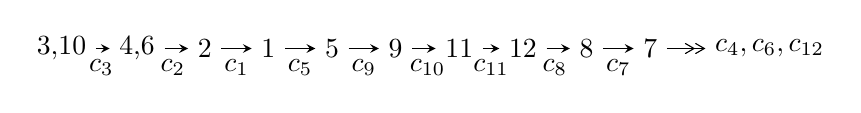
\begin{tikzpicture}[x=23pt, y=7pt]
	% node
	\node (A0) at (-1/8, 0) {3,10};
	\node (A1) at (17/16, 0) {4,6};
	\node (A2) at (17/8, 0) {2};
	\node (A3) at (25/8, 0) {1};
	\node (A4) at (33/8, 0) {5};
	\node (A5) at (41/8, 0) {9};
	\node (A6) at (49/8, 0) {11};
	\node (A7) at (57/8, 0) {12};
	\node (A8) at (65/8, 0) {8};
	\node (A9) at (73/8, 0) {7};
	\node (C1) at (1/2, -1) {$c_{3}$};
	\node (C2) at (13/8, -1) {$c_{2}$};
	\node (C3) at (21/8, -1) {$c_{1}$};
	\node (C4) at (29/8, -1) {$c_{5}$};
	\node (C5) at (37/8, -1) {$c_{9}$};
	\node (C6) at (45/8, -1) {$c_{10}$};
	\node (C7) at (53/8, -1) {$c_{11}$};
	\node (C8) at (61/8, -1) {$c_{8}$};
	\node (C9) at (69/8, -1) {$c_{7}$};
	\node (A10) at (11, 0) {$c_{4},c_{6},c_{12}$};

	% edge
	\draw[->,>=stealth]	
	(A0) edge (A1) (A1) edge (A2) (A2) edge (A3) (A3) edge (A4) (A4) edge (A5) (A5) edge (A6) (A6) edge (A7) (A7) edge (A8) (A8) edge (A9) ;
	\draw[->>,>={angle 60}]	
	(A9) edge (A10);
\end{tikzpicture} \\ 

\end{tabular} \\

\footnotetext{
The image of knot diagram is generated by the software ``\textbf{Draw programme}" developed by Andrew Bartholomew(\url{http://www.layer8.co.uk/maths/draw/index.htm\#Running-draw}), where we modified some parts for our purpose(\url{https://github.com/CATsTAILs/LinksPainter}).
}\phantom \\ \newline 
\centering \textbf{Ideals for irreducible components\footnotemark of $X_{\text{par}}$} 
 
\begin{align*}
I^u_{1}&=\langle 
- u^{41}+u^{40}+\cdots+b+1,\;u^{42}- u^{41}+\cdots+2 a-2,\;u^{43}-3 u^{42}+\cdots+2 u-2\rangle \\
I^u_{2}&=\langle 
-83 u^{30} a+64 u^{30}+\cdots-12 a-29,\;-2 u^{30} a+u^{30}+\cdots-2 a+2,\;u^{31}+u^{30}+\cdots-2 u^2-1\rangle \\
I^u_{3}&=\langle 
b+1,\;u^3-2 u^2+2 a+u,\;u^4+u^2+2\rangle \\
I^u_{4}&=\langle 
b-1,\;a+u-1,\;u^4+1\rangle \\
I^u_{5}&=\langle 
b+1,\;a- u-1,\;u^2+1\rangle \\
\\
I^v_{1}&=\langle 
a,\;b-1,\;v+1\rangle \\
\end{align*}
\raggedright * 6 irreducible components of $\dim_{\mathbb{C}}=0$, with total 116 representations.\\
\footnotetext{All coefficients of polynomials are rational numbers. But the coefficients are sometimes approximated in decimal forms when there is not enough margin.}
\newpage
\renewcommand{\arraystretch}{1}
\centering \section*{I. $I^u_{1}= \langle - u^{41}+u^{40}+\cdots+b+1,\;u^{42}- u^{41}+\cdots+2 a-2,\;u^{43}-3 u^{42}+\cdots+2 u-2 \rangle$}
\flushleft \textbf{(i) Arc colorings}\\
\begin{tabular}{m{7pt} m{180pt} m{7pt} m{180pt} }
\flushright $a_{3}=$&$\begin{pmatrix}1\\0\end{pmatrix}$ \\
\flushright $a_{10}=$&$\begin{pmatrix}0\\u\end{pmatrix}$ \\
\flushright $a_{4}=$&$\begin{pmatrix}1\\u^2\end{pmatrix}$ \\
\flushright $a_{6}=$&$\begin{pmatrix}-\frac{1}{2} u^{42}+\frac{1}{2} u^{41}+\cdots+u+1\\u^{41}- u^{40}+\cdots+3 u^2-1\end{pmatrix}$ \\
\flushright $a_{2}=$&$\begin{pmatrix}-\frac{5}{2} u^{42}+\frac{9}{2} u^{41}+\cdots+u^2+4 u\\- u^{42}+2 u^{41}+\cdots+2 u-1\end{pmatrix}$ \\
\flushright $a_{1}=$&$\begin{pmatrix}-\frac{7}{2} u^{42}+\frac{13}{2} u^{41}+\cdots+6 u-1\\- u^{42}+2 u^{41}+\cdots+2 u-1\end{pmatrix}$ \\
\flushright $a_{5}=$&$\begin{pmatrix}u^{10}+u^8+2 u^6+u^4+u^2+1\\u^{12}+2 u^{10}+4 u^8+4 u^6+3 u^4+2 u^2\end{pmatrix}$ \\
\flushright $a_{9}=$&$\begin{pmatrix}u\\u^3+u\end{pmatrix}$ \\
\flushright $a_{11}=$&$\begin{pmatrix}u^3\\u^5+u^3+u\end{pmatrix}$ \\
\flushright $a_{12}=$&$\begin{pmatrix}-\frac{5}{2} u^{42}+\frac{9}{2} u^{41}+\cdots+4 u-1\\- u^{42}+2 u^{41}+\cdots+3 u-1\end{pmatrix}$ \\
\flushright $a_{8}=$&$\begin{pmatrix}u^5+u\\u^7+u^5+2 u^3+u\end{pmatrix}$ \\
\flushright $a_{7}=$&$\begin{pmatrix}u^{15}+2 u^{13}+4 u^{11}+4 u^9+4 u^7+4 u^5+2 u^3+2 u\\u^{17}+3 u^{15}+7 u^{13}+10 u^{11}+11 u^9+10 u^7+6 u^5+4 u^3+u\end{pmatrix}$\\&\end{tabular}
\flushleft \textbf{(ii) Obstruction class $= -1$}\\~\\
\flushleft \textbf{(iii) Cusp Shapes $= -16 u^{42}+34 u^{41}+\cdots+22 u-20$}\\~\\
\newpage\renewcommand{\arraystretch}{1}
\flushleft \textbf{(iv) u-Polynomials at the component}\newline \\
\begin{tabular}{m{50pt}|m{274pt}}
Crossings & \hspace{64pt}u-Polynomials at each crossing \\
\hline $$\begin{aligned}c_{1},c_{11}\end{aligned}$$&$\begin{aligned}
&u^{43}+17 u^{42}+\cdots+16 u+1
\end{aligned}$\\
\hline $$\begin{aligned}c_{2},c_{5},c_{6}\\c_{12}\end{aligned}$$&$\begin{aligned}
&u^{43}+u^{42}+\cdots-8 u^2+1
\end{aligned}$\\
\hline $$\begin{aligned}c_{3},c_{9}\end{aligned}$$&$\begin{aligned}
&u^{43}+3 u^{42}+\cdots+2 u+2
\end{aligned}$\\
\hline $$\begin{aligned}c_{4},c_{7}\end{aligned}$$&$\begin{aligned}
&u^{43}-15 u^{42}+\cdots-2154 u+158
\end{aligned}$\\
\hline $$\begin{aligned}c_{8},c_{10}\end{aligned}$$&$\begin{aligned}
&u^{43}-15 u^{42}+\cdots+12 u+4
\end{aligned}$\\
\hline
\end{tabular}\\~\\
\newpage\renewcommand{\arraystretch}{1}
\flushleft \textbf{(v) Riley Polynomials at the component}\newline \\
\begin{tabular}{m{50pt}|m{274pt}}
Crossings & \hspace{64pt}Riley Polynomials at each crossing \\
\hline $$\begin{aligned}c_{1},c_{11}\end{aligned}$$&$\begin{aligned}
&y^{43}+31 y^{42}+\cdots+36 y-1
\end{aligned}$\\
\hline $$\begin{aligned}c_{2},c_{5},c_{6}\\c_{12}\end{aligned}$$&$\begin{aligned}
&y^{43}-17 y^{42}+\cdots+16 y-1
\end{aligned}$\\
\hline $$\begin{aligned}c_{3},c_{9}\end{aligned}$$&$\begin{aligned}
&y^{43}+15 y^{42}+\cdots+12 y-4
\end{aligned}$\\
\hline $$\begin{aligned}c_{4},c_{7}\end{aligned}$$&$\begin{aligned}
&y^{43}+27 y^{42}+\cdots+268172 y-24964
\end{aligned}$\\
\hline $$\begin{aligned}c_{8},c_{10}\end{aligned}$$&$\begin{aligned}
&y^{43}+27 y^{42}+\cdots+784 y-16
\end{aligned}$\\
\hline
\end{tabular}\\~\\
\newpage\flushleft \textbf{(vi) Complex Volumes and Cusp Shapes}
$$\begin{array}{c|c|c}  
\text{Solutions to }I^u_{1}& \I (\text{vol} + \sqrt{-1}CS) & \text{Cusp shape}\\
 \hline 
\begin{aligned}
u &= \phantom{-}0.810305 + 0.610083 I \\
a &= -0.872253 - 1.072020 I \\
b &= -1.165720 + 0.639728 I\end{aligned}
 & -0.67916 + 11.73210 I & -10.65839 - 6.76823 I \\ \hline\begin{aligned}
u &= \phantom{-}0.810305 - 0.610083 I \\
a &= -0.872253 + 1.072020 I \\
b &= -1.165720 - 0.639728 I\end{aligned}
 & -0.67916 - 11.73210 I & -10.65839 + 6.76823 I \\ \hline\begin{aligned}
u &= -0.169320 + 0.970646 I \\
a &= \phantom{-}1.076800 + 0.490969 I \\
b &= -0.864916 - 0.541410 I\end{aligned}
 & \phantom{-}1.81117 - 1.96121 I & -3.54414 + 2.58212 I \\ \hline\begin{aligned}
u &= -0.169320 - 0.970646 I \\
a &= \phantom{-}1.076800 - 0.490969 I \\
b &= -0.864916 + 0.541410 I\end{aligned}
 & \phantom{-}1.81117 + 1.96121 I & -3.54414 - 2.58212 I \\ \hline\begin{aligned}
u &= -0.404499 + 0.937684 I \\
a &= -0.09752 - 2.06018 I \\
b &= -1.003290 + 0.619413 I\end{aligned}
 & \phantom{-}0.64091 + 7.57935 I & -5.71587 - 9.06778 I \\ \hline\begin{aligned}
u &= -0.404499 - 0.937684 I \\
a &= -0.09752 + 2.06018 I \\
b &= -1.003290 - 0.619413 I\end{aligned}
 & \phantom{-}0.64091 - 7.57935 I & -5.71587 + 9.06778 I \\ \hline\begin{aligned}
u &= -0.740546 + 0.734320 I \\
a &= \phantom{-}0.953869 + 0.031628 I \\
b &= \phantom{-}0.638692 + 0.127245 I\end{aligned}
 & -3.38498 - 0.54186 I & -9.64597 + 2.59436 I \\ \hline\begin{aligned}
u &= -0.740546 - 0.734320 I \\
a &= \phantom{-}0.953869 - 0.031628 I \\
b &= \phantom{-}0.638692 - 0.127245 I\end{aligned}
 & -3.38498 + 0.54186 I & -9.64597 - 2.59436 I \\ \hline\begin{aligned}
u &= \phantom{-}0.767460 + 0.565351 I \\
a &= \phantom{-}0.203752 + 0.596820 I \\
b &= -0.551586 - 0.826342 I\end{aligned}
 & \phantom{-}3.23658 + 0.48012 I & -5.52727 + 1.98665 I \\ \hline\begin{aligned}
u &= \phantom{-}0.767460 - 0.565351 I \\
a &= \phantom{-}0.203752 - 0.596820 I \\
b &= -0.551586 + 0.826342 I\end{aligned}
 & \phantom{-}3.23658 - 0.48012 I & -5.52727 - 1.98665 I\\
 \hline 
 \end{array}$$\newpage$$\begin{array}{c|c|c}  
\text{Solutions to }I^u_{1}& \I (\text{vol} + \sqrt{-1}CS) & \text{Cusp shape}\\
 \hline 
\begin{aligned}
u &= \phantom{-}0.781599 + 0.706193 I \\
a &= \phantom{-}1.015530 + 0.059356 I \\
b &= \phantom{-}0.943303 + 0.436662 I\end{aligned}
 & -4.27279 - 2.51600 I & -12.07773 + 5.71847 I \\ \hline\begin{aligned}
u &= \phantom{-}0.781599 - 0.706193 I \\
a &= \phantom{-}1.015530 - 0.059356 I \\
b &= \phantom{-}0.943303 - 0.436662 I\end{aligned}
 & -4.27279 + 2.51600 I & -12.07773 - 5.71847 I \\ \hline\begin{aligned}
u &= \phantom{-}0.634409 + 0.863030 I \\
a &= \phantom{-}0.482681 - 0.289079 I \\
b &= -0.073637 + 0.560874 I\end{aligned}
 & -0.87271 - 2.47607 I & -4.48573 + 2.92592 I \\ \hline\begin{aligned}
u &= \phantom{-}0.634409 - 0.863030 I \\
a &= \phantom{-}0.482681 + 0.289079 I \\
b &= -0.073637 - 0.560874 I\end{aligned}
 & -0.87271 + 2.47607 I & -4.48573 - 2.92592 I \\ \hline\begin{aligned}
u &= -0.730178 + 0.509618 I \\
a &= \phantom{-}0.210279 + 0.671513 I \\
b &= -0.659249 - 0.796369 I\end{aligned}
 & \phantom{-}3.58914 - 2.18174 I & -5.59185 + 2.68261 I \\ \hline\begin{aligned}
u &= -0.730178 - 0.509618 I \\
a &= \phantom{-}0.210279 - 0.671513 I \\
b &= -0.659249 + 0.796369 I\end{aligned}
 & \phantom{-}3.58914 + 2.18174 I & -5.59185 - 2.68261 I \\ \hline\begin{aligned}
u &= \phantom{-}0.064317 + 0.887781 I \\
a &= \phantom{-}0.245081 + 0.904782 I \\
b &= -0.514108 - 0.340137 I\end{aligned}
 & \phantom{-}1.82719 - 1.38027 I & -1.41434 + 5.67019 I \\ \hline\begin{aligned}
u &= \phantom{-}0.064317 - 0.887781 I \\
a &= \phantom{-}0.245081 - 0.904782 I \\
b &= -0.514108 + 0.340137 I\end{aligned}
 & \phantom{-}1.82719 + 1.38027 I & -1.41434 - 5.67019 I \\ \hline\begin{aligned}
u &= -0.019617 + 1.114870 I \\
a &= -1.21478 - 1.96630 I \\
b &= \phantom{-}0.614989 + 0.851882 I\end{aligned}
 & \phantom{-}8.98390 - 0.70392 I & \phantom{-}0.62643 + 2.07043 I \\ \hline\begin{aligned}
u &= -0.019617 - 1.114870 I \\
a &= -1.21478 + 1.96630 I \\
b &= \phantom{-}0.614989 - 0.851882 I\end{aligned}
 & \phantom{-}8.98390 + 0.70392 I & \phantom{-}0.62643 - 2.07043 I\\
 \hline 
 \end{array}$$\newpage$$\begin{array}{c|c|c}  
\text{Solutions to }I^u_{1}& \I (\text{vol} + \sqrt{-1}CS) & \text{Cusp shape}\\
 \hline 
\begin{aligned}
u &= -0.070568 + 1.113790 I \\
a &= -0.93313 + 2.40704 I \\
b &= \phantom{-}1.150350 - 0.663782 I\end{aligned}
 & \phantom{-}5.52719 + 10.86160 I & -3.74256 - 7.47837 I \\ \hline\begin{aligned}
u &= -0.070568 - 1.113790 I \\
a &= -0.93313 - 2.40704 I \\
b &= \phantom{-}1.150350 + 0.663782 I\end{aligned}
 & \phantom{-}5.52719 - 10.86160 I & -3.74256 + 7.47837 I \\ \hline\begin{aligned}
u &= \phantom{-}0.769424 + 0.820046 I \\
a &= \phantom{-}1.203010 - 0.319741 I \\
b &= \phantom{-}1.082070 - 0.520953 I\end{aligned}
 & -6.01940 + 4.69142 I & -13.7584 - 4.2985 I \\ \hline\begin{aligned}
u &= \phantom{-}0.769424 - 0.820046 I \\
a &= \phantom{-}1.203010 + 0.319741 I \\
b &= \phantom{-}1.082070 + 0.520953 I\end{aligned}
 & -6.01940 - 4.69142 I & -13.7584 + 4.2985 I \\ \hline\begin{aligned}
u &= \phantom{-}0.747584 + 0.908886 I \\
a &= -1.77260 + 1.30694 I \\
b &= -1.099080 - 0.534938 I\end{aligned}
 & -5.74879 - 10.41320 I & -13.1188 + 9.7708 I \\ \hline\begin{aligned}
u &= \phantom{-}0.747584 - 0.908886 I \\
a &= -1.77260 - 1.30694 I \\
b &= -1.099080 + 0.534938 I\end{aligned}
 & -5.74879 + 10.41320 I & -13.1188 - 9.7708 I \\ \hline\begin{aligned}
u &= -0.587598 + 1.034130 I \\
a &= -0.976042 - 0.394281 I \\
b &= \phantom{-}1.109900 + 0.674647 I\end{aligned}
 & \phantom{-}2.34669 - 4.11995 I & -6.41118 + 2.08920 I \\ \hline\begin{aligned}
u &= -0.587598 - 1.034130 I \\
a &= -0.976042 + 0.394281 I \\
b &= \phantom{-}1.109900 - 0.674647 I\end{aligned}
 & \phantom{-}2.34669 + 4.11995 I & -6.41118 - 2.08920 I \\ \hline\begin{aligned}
u &= -0.697004 + 0.966572 I \\
a &= -0.886537 - 0.919821 I \\
b &= -0.663489 + 0.163610 I\end{aligned}
 & -2.67878 + 6.02819 I & -8.00000 - 8.68993 I \\ \hline\begin{aligned}
u &= -0.697004 - 0.966572 I \\
a &= -0.886537 + 0.919821 I \\
b &= -0.663489 - 0.163610 I\end{aligned}
 & -2.67878 - 6.02819 I & -8.00000 + 8.68993 I\\
 \hline 
 \end{array}$$\newpage$$\begin{array}{c|c|c}  
\text{Solutions to }I^u_{1}& \I (\text{vol} + \sqrt{-1}CS) & \text{Cusp shape}\\
 \hline 
\begin{aligned}
u &= -0.693381 + 0.387489 I \\
a &= -0.79741 - 1.27275 I \\
b &= -1.120710 + 0.646264 I\end{aligned}
 & \phantom{-}0.58526 + 8.92556 I & -9.86563 - 7.36810 I \\ \hline\begin{aligned}
u &= -0.693381 - 0.387489 I \\
a &= -0.79741 + 1.27275 I \\
b &= -1.120710 - 0.646264 I\end{aligned}
 & \phantom{-}0.58526 - 8.92556 I & -9.86563 + 7.36810 I \\ \hline\begin{aligned}
u &= \phantom{-}0.710991 + 0.990924 I \\
a &= -0.093051 + 1.044480 I \\
b &= -0.922866 + 0.415678 I\end{aligned}
 & -3.40970 - 3.12696 I & -10.17371 + 0. I\phantom{ +0.000000I} \\ \hline\begin{aligned}
u &= \phantom{-}0.710991 - 0.990924 I \\
a &= -0.093051 - 1.044480 I \\
b &= -0.922866 - 0.415678 I\end{aligned}
 & -3.40970 + 3.12696 I & -10.17371 + 0. I\phantom{ +0.000000I} \\ \hline\begin{aligned}
u &= -0.635885 + 1.042150 I \\
a &= \phantom{-}0.39218 + 2.01011 I \\
b &= \phantom{-}0.683334 - 0.830391 I\end{aligned}
 & \phantom{-}5.11017 + 7.38861 I & -3.39621 - 7.50854 I \\ \hline\begin{aligned}
u &= -0.635885 - 1.042150 I \\
a &= \phantom{-}0.39218 - 2.01011 I \\
b &= \phantom{-}0.683334 + 0.830391 I\end{aligned}
 & \phantom{-}5.11017 - 7.38861 I & -3.39621 + 7.50854 I \\ \hline\begin{aligned}
u &= \phantom{-}0.663748 + 1.042840 I \\
a &= -1.50776 + 0.41692 I \\
b &= \phantom{-}0.546956 - 0.859893 I\end{aligned}
 & \phantom{-}4.63845 - 5.90595 I & -3.49620 + 2.84362 I \\ \hline\begin{aligned}
u &= \phantom{-}0.663748 - 1.042840 I \\
a &= -1.50776 - 0.41692 I \\
b &= \phantom{-}0.546956 + 0.859893 I\end{aligned}
 & \phantom{-}4.63845 + 5.90595 I & -3.49620 - 2.84362 I \\ \hline\begin{aligned}
u &= \phantom{-}0.692059 + 1.043830 I \\
a &= \phantom{-}1.02365 - 2.73608 I \\
b &= \phantom{-}1.174490 + 0.646634 I\end{aligned}
 & \phantom{-}0.6235 - 17.3797 I & -8.00000 + 11.25544 I \\ \hline\begin{aligned}
u &= \phantom{-}0.692059 - 1.043830 I \\
a &= \phantom{-}1.02365 + 2.73608 I \\
b &= \phantom{-}1.174490 - 0.646634 I\end{aligned}
 & \phantom{-}0.6235 + 17.3797 I & -8.00000 - 11.25544 I\\
 \hline 
 \end{array}$$\newpage$$\begin{array}{c|c|c}  
\text{Solutions to }I^u_{1}& \I (\text{vol} + \sqrt{-1}CS) & \text{Cusp shape}\\
 \hline 
\begin{aligned}
u &= -0.580815 + 0.131701 I \\
a &= \phantom{-}0.893430 + 0.128520 I \\
b &= \phantom{-}0.976159 + 0.538801 I\end{aligned}
 & -1.61575 - 4.22948 I & -11.92293 + 4.59304 I \\ \hline\begin{aligned}
u &= -0.580815 - 0.131701 I \\
a &= \phantom{-}0.893430 - 0.128520 I \\
b &= \phantom{-}0.976159 - 0.538801 I\end{aligned}
 & -1.61575 + 4.22948 I & -11.92293 - 4.59304 I \\ \hline\begin{aligned}
u &= \phantom{-}0.375038\phantom{ +0.000000I} \\
a &= \phantom{-}0.901679\phantom{ +0.000000I} \\
b &= \phantom{-}0.436822\phantom{ +0.000000I}\end{aligned}
 & -0.737041\phantom{ +0.000000I} & -13.3130\phantom{ +0.000000I}\\
 \hline 
 \end{array}$$\newpage\newpage\renewcommand{\arraystretch}{1}
\centering \section*{II. $I^u_{2}= \langle -83 u^{30} a+64 u^{30}+\cdots-12 a-29,\;-2 u^{30} a+u^{30}+\cdots-2 a+2,\;u^{31}+u^{30}+\cdots-2 u^2-1 \rangle$}
\flushleft \textbf{(i) Arc colorings}\\
\begin{tabular}{m{7pt} m{180pt} m{7pt} m{180pt} }
\flushright $a_{3}=$&$\begin{pmatrix}1\\0\end{pmatrix}$ \\
\flushright $a_{10}=$&$\begin{pmatrix}0\\u\end{pmatrix}$ \\
\flushright $a_{4}=$&$\begin{pmatrix}1\\u^2\end{pmatrix}$ \\
\flushright $a_{6}=$&$\begin{pmatrix}a\\1.66000 a u^{30}-1.28000 u^{30}+\cdots+0.240000 a+0.580000\end{pmatrix}$ \\
\flushright $a_{2}=$&$\begin{pmatrix}-1.28000 a u^{30}+1.74000 u^{30}+\cdots+0.580000 a-0.140000\\-1.52000 a u^{30}+1.66000 u^{30}+\cdots-0.780000 a-0.760000\end{pmatrix}$ \\
\flushright $a_{1}=$&$\begin{pmatrix}-2.80000 a u^{30}+3.40000 u^{30}+\cdots-0.200000 a-0.900000\\-1.52000 a u^{30}+1.66000 u^{30}+\cdots-0.780000 a-0.760000\end{pmatrix}$ \\
\flushright $a_{5}=$&$\begin{pmatrix}u^{10}+u^8+2 u^6+u^4+u^2+1\\u^{12}+2 u^{10}+4 u^8+4 u^6+3 u^4+2 u^2\end{pmatrix}$ \\
\flushright $a_{9}=$&$\begin{pmatrix}u\\u^3+u\end{pmatrix}$ \\
\flushright $a_{11}=$&$\begin{pmatrix}u^3\\u^5+u^3+u\end{pmatrix}$ \\
\flushright $a_{12}=$&$\begin{pmatrix}1.28000 a u^{30}-1.74000 u^{30}+\cdots-0.580000 a+1.14000\\1\end{pmatrix}$ \\
\flushright $a_{8}=$&$\begin{pmatrix}u^5+u\\u^7+u^5+2 u^3+u\end{pmatrix}$ \\
\flushright $a_{7}=$&$\begin{pmatrix}u^{15}+2 u^{13}+4 u^{11}+4 u^9+4 u^7+4 u^5+2 u^3+2 u\\u^{17}+3 u^{15}+7 u^{13}+10 u^{11}+11 u^9+10 u^7+6 u^5+4 u^3+u\end{pmatrix}$\\&\end{tabular}
\flushleft \textbf{(ii) Obstruction class $= -1$}\\~\\
\flushleft \textbf{(iii) Cusp Shapes $= 4 u^{30}+20 u^{28}-4 u^{27}+68 u^{26}-20 u^{25}+160 u^{24}-64 u^{23}+300 u^{22}-144 u^{21}+460 u^{20}-252 u^{19}+592 u^{18}-364 u^{17}+660 u^{16}-436 u^{15}+628 u^{14}-452 u^{13}+528 u^{12}-396 u^{11}+380 u^{10}-296 u^9+236 u^8-188 u^7+128 u^6-92 u^5+52 u^4-40 u^3+20 u^2-12 u-6$}\\~\\
\newpage\renewcommand{\arraystretch}{1}
\flushleft \textbf{(iv) u-Polynomials at the component}\newline \\
\begin{tabular}{m{50pt}|m{274pt}}
Crossings & \hspace{64pt}u-Polynomials at each crossing \\
\hline $$\begin{aligned}c_{1},c_{11}\end{aligned}$$&$\begin{aligned}
&u^{62}+33 u^{61}+\cdots+2505 u+256
\end{aligned}$\\
\hline $$\begin{aligned}c_{2},c_{5},c_{6}\\c_{12}\end{aligned}$$&$\begin{aligned}
&u^{62}+u^{61}+\cdots+19 u+16
\end{aligned}$\\
\hline $$\begin{aligned}c_{3},c_{9}\end{aligned}$$&$\begin{aligned}
&(u^{31}- u^{30}+\cdots+2 u^2+1)^{2}
\end{aligned}$\\
\hline $$\begin{aligned}c_{4},c_{7}\end{aligned}$$&$\begin{aligned}
&(u^{31}+5 u^{30}+\cdots+40 u+7)^{2}
\end{aligned}$\\
\hline $$\begin{aligned}c_{8},c_{10}\end{aligned}$$&$\begin{aligned}
&(u^{31}-11 u^{30}+\cdots-4 u+1)^{2}
\end{aligned}$\\
\hline
\end{tabular}\\~\\
\newpage\renewcommand{\arraystretch}{1}
\flushleft \textbf{(v) Riley Polynomials at the component}\newline \\
\begin{tabular}{m{50pt}|m{274pt}}
Crossings & \hspace{64pt}Riley Polynomials at each crossing \\
\hline $$\begin{aligned}c_{1},c_{11}\end{aligned}$$&$\begin{aligned}
&y^{62}-9 y^{61}+\cdots+636463 y+65536
\end{aligned}$\\
\hline $$\begin{aligned}c_{2},c_{5},c_{6}\\c_{12}\end{aligned}$$&$\begin{aligned}
&y^{62}-33 y^{61}+\cdots-2505 y+256
\end{aligned}$\\
\hline $$\begin{aligned}c_{3},c_{9}\end{aligned}$$&$\begin{aligned}
&(y^{31}+11 y^{30}+\cdots-4 y-1)^{2}
\end{aligned}$\\
\hline $$\begin{aligned}c_{4},c_{7}\end{aligned}$$&$\begin{aligned}
&(y^{31}+23 y^{30}+\cdots-640 y-49)^{2}
\end{aligned}$\\
\hline $$\begin{aligned}c_{8},c_{10}\end{aligned}$$&$\begin{aligned}
&(y^{31}+19 y^{30}+\cdots-8 y-1)^{2}
\end{aligned}$\\
\hline
\end{tabular}\\~\\
\newpage\flushleft \textbf{(vi) Complex Volumes and Cusp Shapes}
$$\begin{array}{c|c|c}  
\text{Solutions to }I^u_{2}& \I (\text{vol} + \sqrt{-1}CS) & \text{Cusp shape}\\
 \hline 
\begin{aligned}
u &= -0.794006 + 0.593785 I \\
a &= -0.575606 + 1.111050 I \\
b &= -1.060010 - 0.663363 I\end{aligned}
 & \phantom{-}1.70250 - 6.04082 I & -7.64635 + 3.16093 I \\ \hline\begin{aligned}
u &= -0.794006 + 0.593785 I \\
a &= \phantom{-}0.268388 - 0.355056 I \\
b &= -0.378076 + 0.912441 I\end{aligned}
 & \phantom{-}1.70250 - 6.04082 I & -7.64635 + 3.16093 I \\ \hline\begin{aligned}
u &= -0.794006 - 0.593785 I \\
a &= -0.575606 - 1.111050 I \\
b &= -1.060010 + 0.663363 I\end{aligned}
 & \phantom{-}1.70250 + 6.04082 I & -7.64635 - 3.16093 I \\ \hline\begin{aligned}
u &= -0.794006 - 0.593785 I \\
a &= \phantom{-}0.268388 + 0.355056 I \\
b &= -0.378076 - 0.912441 I\end{aligned}
 & \phantom{-}1.70250 + 6.04082 I & -7.64635 - 3.16093 I \\ \hline\begin{aligned}
u &= \phantom{-}0.752643 + 0.616875 I \\
a &= \phantom{-}1.049010 - 0.024204 I \\
b &= \phantom{-}1.292420 + 0.176912 I\end{aligned}
 & -4.01963 + 2.73446 I & -11.76690 - 3.38925 I \\ \hline\begin{aligned}
u &= \phantom{-}0.752643 + 0.616875 I \\
a &= -0.19620 - 1.79030 I \\
b &= -0.948917 + 0.478047 I\end{aligned}
 & -4.01963 + 2.73446 I & -11.76690 - 3.38925 I \\ \hline\begin{aligned}
u &= \phantom{-}0.752643 - 0.616875 I \\
a &= \phantom{-}1.049010 + 0.024204 I \\
b &= \phantom{-}1.292420 - 0.176912 I\end{aligned}
 & -4.01963 - 2.73446 I & -11.76690 + 3.38925 I \\ \hline\begin{aligned}
u &= \phantom{-}0.752643 - 0.616875 I \\
a &= -0.19620 + 1.79030 I \\
b &= -0.948917 - 0.478047 I\end{aligned}
 & -4.01963 - 2.73446 I & -11.76690 + 3.38925 I \\ \hline\begin{aligned}
u &= \phantom{-}0.307711 + 0.890519 I \\
a &= \phantom{-}0.991470 - 0.636002 I \\
b &= -0.548491 + 0.670065 I\end{aligned}
 & \phantom{-}1.93424 - 2.56488 I & -2.83547 + 4.43258 I \\ \hline\begin{aligned}
u &= \phantom{-}0.307711 + 0.890519 I \\
a &= \phantom{-}0.06449 + 1.90945 I \\
b &= -0.810066 - 0.589243 I\end{aligned}
 & \phantom{-}1.93424 - 2.56488 I & -2.83547 + 4.43258 I\\
 \hline 
 \end{array}$$\newpage$$\begin{array}{c|c|c}  
\text{Solutions to }I^u_{2}& \I (\text{vol} + \sqrt{-1}CS) & \text{Cusp shape}\\
 \hline 
\begin{aligned}
u &= \phantom{-}0.307711 - 0.890519 I \\
a &= \phantom{-}0.991470 + 0.636002 I \\
b &= -0.548491 - 0.670065 I\end{aligned}
 & \phantom{-}1.93424 + 2.56488 I & -2.83547 - 4.43258 I \\ \hline\begin{aligned}
u &= \phantom{-}0.307711 - 0.890519 I \\
a &= \phantom{-}0.06449 - 1.90945 I \\
b &= -0.810066 + 0.589243 I\end{aligned}
 & \phantom{-}1.93424 + 2.56488 I & -2.83547 - 4.43258 I \\ \hline\begin{aligned}
u &= -0.028596 + 1.074730 I \\
a &= \phantom{-}1.254810 + 0.086042 I \\
b &= -1.300190 - 0.121437 I\end{aligned}
 & \phantom{-}1.60703 + 1.99617 I & -4.10076 - 3.62729 I \\ \hline\begin{aligned}
u &= -0.028596 + 1.074730 I \\
a &= -1.60467 + 2.59295 I \\
b &= \phantom{-}0.865196 - 0.489813 I\end{aligned}
 & \phantom{-}1.60703 + 1.99617 I & -4.10076 - 3.62729 I \\ \hline\begin{aligned}
u &= -0.028596 - 1.074730 I \\
a &= \phantom{-}1.254810 - 0.086042 I \\
b &= -1.300190 + 0.121437 I\end{aligned}
 & \phantom{-}1.60703 - 1.99617 I & -4.10076 + 3.62729 I \\ \hline\begin{aligned}
u &= -0.028596 - 1.074730 I \\
a &= -1.60467 - 2.59295 I \\
b &= \phantom{-}0.865196 + 0.489813 I\end{aligned}
 & \phantom{-}1.60703 - 1.99617 I & -4.10076 + 3.62729 I \\ \hline\begin{aligned}
u &= -0.730031 + 0.790482 I \\
a &= \phantom{-}1.124130 + 0.092019 I \\
b &= \phantom{-}0.982872 + 0.347185 I\end{aligned}
 & -3.79282 - 0.40298 I & -11.07070 + 0.52831 I \\ \hline\begin{aligned}
u &= -0.730031 + 0.790482 I \\
a &= \phantom{-}0.801595 - 0.042941 I \\
b &= \phantom{-}0.213919 - 0.536430 I\end{aligned}
 & -3.79282 - 0.40298 I & -11.07070 + 0.52831 I \\ \hline\begin{aligned}
u &= -0.730031 - 0.790482 I \\
a &= \phantom{-}1.124130 - 0.092019 I \\
b &= \phantom{-}0.982872 - 0.347185 I\end{aligned}
 & -3.79282 + 0.40298 I & -11.07070 - 0.52831 I \\ \hline\begin{aligned}
u &= -0.730031 - 0.790482 I \\
a &= \phantom{-}0.801595 + 0.042941 I \\
b &= \phantom{-}0.213919 + 0.536430 I\end{aligned}
 & -3.79282 + 0.40298 I & -11.07070 - 0.52831 I\\
 \hline 
 \end{array}$$\newpage$$\begin{array}{c|c|c}  
\text{Solutions to }I^u_{2}& \I (\text{vol} + \sqrt{-1}CS) & \text{Cusp shape}\\
 \hline 
\begin{aligned}
u &= \phantom{-}0.709633 + 0.857826 I \\
a &= \phantom{-}1.50924 + 0.06570 I \\
b &= \phantom{-}1.162280 - 0.314153 I\end{aligned}
 & -7.28578 - 2.71284 I & -15.8994 + 3.4466 I \\ \hline\begin{aligned}
u &= \phantom{-}0.709633 + 0.857826 I \\
a &= -1.89841 + 2.00937 I \\
b &= -1.134280 - 0.338014 I\end{aligned}
 & -7.28578 - 2.71284 I & -15.8994 + 3.4466 I \\ \hline\begin{aligned}
u &= \phantom{-}0.709633 - 0.857826 I \\
a &= \phantom{-}1.50924 - 0.06570 I \\
b &= \phantom{-}1.162280 + 0.314153 I\end{aligned}
 & -7.28578 + 2.71284 I & -15.8994 - 3.4466 I \\ \hline\begin{aligned}
u &= \phantom{-}0.709633 - 0.857826 I \\
a &= -1.89841 - 2.00937 I \\
b &= -1.134280 + 0.338014 I\end{aligned}
 & -7.28578 + 2.71284 I & -15.8994 - 3.4466 I \\ \hline\begin{aligned}
u &= \phantom{-}0.048600 + 1.113390 I \\
a &= -1.10147 + 1.83797 I \\
b &= \phantom{-}0.429611 - 0.922254 I\end{aligned}
 & \phantom{-}7.71400 - 5.04935 I & -0.87471 + 3.42516 I \\ \hline\begin{aligned}
u &= \phantom{-}0.048600 + 1.113390 I \\
a &= -1.08873 - 2.37779 I \\
b &= \phantom{-}1.032690 + 0.699331 I\end{aligned}
 & \phantom{-}7.71400 - 5.04935 I & -0.87471 + 3.42516 I \\ \hline\begin{aligned}
u &= \phantom{-}0.048600 - 1.113390 I \\
a &= -1.10147 - 1.83797 I \\
b &= \phantom{-}0.429611 + 0.922254 I\end{aligned}
 & \phantom{-}7.71400 + 5.04935 I & -0.87471 - 3.42516 I \\ \hline\begin{aligned}
u &= \phantom{-}0.048600 - 1.113390 I \\
a &= -1.08873 + 2.37779 I \\
b &= \phantom{-}1.032690 - 0.699331 I\end{aligned}
 & \phantom{-}7.71400 + 5.04935 I & -0.87471 - 3.42516 I \\ \hline\begin{aligned}
u &= -0.630136 + 0.611565 I \\
a &= \phantom{-}0.979082 + 0.056700 I \\
b &= \phantom{-}1.231410 + 0.064735 I\end{aligned}
 & -3.29780 + 0.92992 I & -9.59628 - 3.68841 I \\ \hline\begin{aligned}
u &= -0.630136 + 0.611565 I \\
a &= \phantom{-}0.90502 - 1.81588 I \\
b &= -0.766634 + 0.363749 I\end{aligned}
 & -3.29780 + 0.92992 I & -9.59628 - 3.68841 I\\
 \hline 
 \end{array}$$\newpage$$\begin{array}{c|c|c}  
\text{Solutions to }I^u_{2}& \I (\text{vol} + \sqrt{-1}CS) & \text{Cusp shape}\\
 \hline 
\begin{aligned}
u &= -0.630136 - 0.611565 I \\
a &= \phantom{-}0.979082 - 0.056700 I \\
b &= \phantom{-}1.231410 - 0.064735 I\end{aligned}
 & -3.29780 - 0.92992 I & -9.59628 + 3.68841 I \\ \hline\begin{aligned}
u &= -0.630136 - 0.611565 I \\
a &= \phantom{-}0.90502 + 1.81588 I \\
b &= -0.766634 - 0.363749 I\end{aligned}
 & -3.29780 - 0.92992 I & -9.59628 + 3.68841 I \\ \hline\begin{aligned}
u &= -0.711244 + 0.915096 I \\
a &= \phantom{-}0.223384 - 0.239937 I \\
b &= -0.229078 - 0.626885 I\end{aligned}
 & -3.41810 + 5.89464 I & -10.05487 - 6.44091 I \\ \hline\begin{aligned}
u &= -0.711244 + 0.915096 I \\
a &= -1.45569 - 1.48316 I \\
b &= -1.009990 + 0.409220 I\end{aligned}
 & -3.41810 + 5.89464 I & -10.05487 - 6.44091 I \\ \hline\begin{aligned}
u &= -0.711244 - 0.915096 I \\
a &= \phantom{-}0.223384 + 0.239937 I \\
b &= -0.229078 + 0.626885 I\end{aligned}
 & -3.41810 - 5.89464 I & -10.05487 + 6.44091 I \\ \hline\begin{aligned}
u &= -0.711244 - 0.915096 I \\
a &= -1.45569 + 1.48316 I \\
b &= -1.009990 - 0.409220 I\end{aligned}
 & -3.41810 - 5.89464 I & -10.05487 + 6.44091 I \\ \hline\begin{aligned}
u &= \phantom{-}0.696118 + 0.446614 I \\
a &= -0.429932 + 1.245830 I \\
b &= -0.983943 - 0.673017 I\end{aligned}
 & \phantom{-}2.60250 - 3.33239 I & -6.76330 + 3.21859 I \\ \hline\begin{aligned}
u &= \phantom{-}0.696118 + 0.446614 I \\
a &= \phantom{-}0.375203 - 0.425155 I \\
b &= -0.451734 + 0.862793 I\end{aligned}
 & \phantom{-}2.60250 - 3.33239 I & -6.76330 + 3.21859 I \\ \hline\begin{aligned}
u &= \phantom{-}0.696118 - 0.446614 I \\
a &= -0.429932 - 1.245830 I \\
b &= -0.983943 + 0.673017 I\end{aligned}
 & \phantom{-}2.60250 + 3.33239 I & -6.76330 - 3.21859 I \\ \hline\begin{aligned}
u &= \phantom{-}0.696118 - 0.446614 I \\
a &= \phantom{-}0.375203 + 0.425155 I \\
b &= -0.451734 - 0.862793 I\end{aligned}
 & \phantom{-}2.60250 + 3.33239 I & -6.76330 - 3.21859 I\\
 \hline 
 \end{array}$$\newpage$$\begin{array}{c|c|c}  
\text{Solutions to }I^u_{2}& \I (\text{vol} + \sqrt{-1}CS) & \text{Cusp shape}\\
 \hline 
\begin{aligned}
u &= -0.642253 + 1.006370 I \\
a &= -0.28971 - 1.62874 I \\
b &= -1.280510 + 0.056589 I\end{aligned}
 & -2.14842 + 4.14236 I & -7.79961 - 2.04013 I \\ \hline\begin{aligned}
u &= -0.642253 + 1.006370 I \\
a &= -1.61379 - 0.81510 I \\
b &= \phantom{-}0.751258 + 0.461288 I\end{aligned}
 & -2.14842 + 4.14236 I & -7.79961 - 2.04013 I \\ \hline\begin{aligned}
u &= -0.642253 - 1.006370 I \\
a &= -0.28971 + 1.62874 I \\
b &= -1.280510 - 0.056589 I\end{aligned}
 & -2.14842 - 4.14236 I & -7.79961 + 2.04013 I \\ \hline\begin{aligned}
u &= -0.642253 - 1.006370 I \\
a &= -1.61379 + 0.81510 I \\
b &= \phantom{-}0.751258 - 0.461288 I\end{aligned}
 & -2.14842 - 4.14236 I & -7.79961 + 2.04013 I \\ \hline\begin{aligned}
u &= \phantom{-}0.611328 + 1.036450 I \\
a &= -1.171880 + 0.475269 I \\
b &= \phantom{-}0.974751 - 0.714129 I\end{aligned}
 & \phantom{-}4.22211 - 1.64856 I & -3.98491 + 2.12263 I \\ \hline\begin{aligned}
u &= \phantom{-}0.611328 + 1.036450 I \\
a &= \phantom{-}0.40901 - 1.68159 I \\
b &= \phantom{-}0.489978 + 0.891236 I\end{aligned}
 & \phantom{-}4.22211 - 1.64856 I & -3.98491 + 2.12263 I \\ \hline\begin{aligned}
u &= \phantom{-}0.611328 - 1.036450 I \\
a &= -1.171880 - 0.475269 I \\
b &= \phantom{-}0.974751 + 0.714129 I\end{aligned}
 & \phantom{-}4.22211 + 1.64856 I & -3.98491 - 2.12263 I \\ \hline\begin{aligned}
u &= \phantom{-}0.611328 - 1.036450 I \\
a &= \phantom{-}0.40901 + 1.68159 I \\
b &= \phantom{-}0.489978 - 0.891236 I\end{aligned}
 & \phantom{-}4.22211 + 1.64856 I & -3.98491 - 2.12263 I \\ \hline\begin{aligned}
u &= \phantom{-}0.673649 + 1.023570 I \\
a &= -0.12488 + 1.47943 I \\
b &= -1.314250 + 0.172694 I\end{aligned}
 & -2.81425 - 8.17190 I & -9.55732 + 8.00325 I \\ \hline\begin{aligned}
u &= \phantom{-}0.673649 + 1.023570 I \\
a &= \phantom{-}0.29874 - 3.07399 I \\
b &= \phantom{-}0.942920 + 0.509265 I\end{aligned}
 & -2.81425 - 8.17190 I & -9.55732 + 8.00325 I\\
 \hline 
 \end{array}$$\newpage$$\begin{array}{c|c|c}  
\text{Solutions to }I^u_{2}& \I (\text{vol} + \sqrt{-1}CS) & \text{Cusp shape}\\
 \hline 
\begin{aligned}
u &= \phantom{-}0.673649 - 1.023570 I \\
a &= -0.12488 - 1.47943 I \\
b &= -1.314250 - 0.172694 I\end{aligned}
 & -2.81425 + 8.17190 I & -9.55732 - 8.00325 I \\ \hline\begin{aligned}
u &= \phantom{-}0.673649 - 1.023570 I \\
a &= \phantom{-}0.29874 + 3.07399 I \\
b &= \phantom{-}0.942920 - 0.509265 I\end{aligned}
 & -2.81425 + 8.17190 I & -9.55732 - 8.00325 I \\ \hline\begin{aligned}
u &= -0.680810 + 1.043630 I \\
a &= -1.54320 - 0.40737 I \\
b &= \phantom{-}0.377634 + 0.934666 I\end{aligned}
 & \phantom{-}3.04348 + 11.60290 I & -5.65053 - 7.70694 I \\ \hline\begin{aligned}
u &= -0.680810 + 1.043630 I \\
a &= \phantom{-}0.80613 + 2.68508 I \\
b &= \phantom{-}1.073030 - 0.677122 I\end{aligned}
 & \phantom{-}3.04348 + 11.60290 I & -5.65053 - 7.70694 I \\ \hline\begin{aligned}
u &= -0.680810 - 1.043630 I \\
a &= -1.54320 + 0.40737 I \\
b &= \phantom{-}0.377634 - 0.934666 I\end{aligned}
 & \phantom{-}3.04348 - 11.60290 I & -5.65053 + 7.70694 I \\ \hline\begin{aligned}
u &= -0.680810 - 1.043630 I \\
a &= \phantom{-}0.80613 - 2.68508 I \\
b &= \phantom{-}1.073030 + 0.677122 I\end{aligned}
 & \phantom{-}3.04348 - 11.60290 I & -5.65053 + 7.70694 I \\ \hline\begin{aligned}
u &= -0.330533 + 0.488116 I \\
a &= \phantom{-}1.010390 + 0.142244 I \\
b &= \phantom{-}1.168370 + 0.123140 I\end{aligned}
 & -3.18273 + 1.02630 I & -10.18992 - 6.41690 I \\ \hline\begin{aligned}
u &= -0.330533 + 0.488116 I \\
a &= \phantom{-}0.66597 - 3.17396 I \\
b &= -0.903345 + 0.276517 I\end{aligned}
 & -3.18273 + 1.02630 I & -10.18992 - 6.41690 I \\ \hline\begin{aligned}
u &= -0.330533 - 0.488116 I \\
a &= \phantom{-}1.010390 - 0.142244 I \\
b &= \phantom{-}1.168370 - 0.123140 I\end{aligned}
 & -3.18273 - 1.02630 I & -10.18992 + 6.41690 I \\ \hline\begin{aligned}
u &= -0.330533 - 0.488116 I \\
a &= \phantom{-}0.66597 + 3.17396 I \\
b &= -0.903345 - 0.276517 I\end{aligned}
 & -3.18273 - 1.02630 I & -10.18992 + 6.41690 I\\
 \hline 
 \end{array}$$\newpage$$\begin{array}{c|c|c}  
\text{Solutions to }I^u_{2}& \I (\text{vol} + \sqrt{-1}CS) & \text{Cusp shape}\\
 \hline 
\begin{aligned}
u &= \phantom{-}0.495857\phantom{ +0.000000I} \\
a &= \phantom{-}0.858117 + 0.046148 I \\
b &= \phantom{-}0.631170 + 0.441733 I\end{aligned}
 & -0.537061\phantom{ +0.000000I} & -10.4180\phantom{ +0.000000I} \\ \hline\begin{aligned}
u &= \phantom{-}0.495857\phantom{ +0.000000I} \\
a &= \phantom{-}0.858117 - 0.046148 I \\
b &= \phantom{-}0.631170 - 0.441733 I\end{aligned}
 & -0.537061\phantom{ +0.000000I} & -10.4180\phantom{ +0.000000I}\\
 \hline 
 \end{array}$$\newpage\newpage\renewcommand{\arraystretch}{1}
\centering \section*{III. $I^u_{3}= \langle b+1,\;u^3-2 u^2+2 a+u,\;u^4+u^2+2 \rangle$}
\flushleft \textbf{(i) Arc colorings}\\
\begin{tabular}{m{7pt} m{180pt} m{7pt} m{180pt} }
\flushright $a_{3}=$&$\begin{pmatrix}1\\0\end{pmatrix}$ \\
\flushright $a_{10}=$&$\begin{pmatrix}0\\u\end{pmatrix}$ \\
\flushright $a_{4}=$&$\begin{pmatrix}1\\u^2\end{pmatrix}$ \\
\flushright $a_{6}=$&$\begin{pmatrix}-\frac{1}{2} u^3+u^2-\frac{1}{2} u\\-1\end{pmatrix}$ \\
\flushright $a_{2}=$&$\begin{pmatrix}-\frac{1}{2} u^3+u^2-\frac{1}{2} u+1\\-1\end{pmatrix}$ \\
\flushright $a_{1}=$&$\begin{pmatrix}-\frac{1}{2} u^3+u^2-\frac{1}{2} u\\-1\end{pmatrix}$ \\
\flushright $a_{5}=$&$\begin{pmatrix}-1\\0\end{pmatrix}$ \\
\flushright $a_{9}=$&$\begin{pmatrix}u\\u^3+u\end{pmatrix}$ \\
\flushright $a_{11}=$&$\begin{pmatrix}u^3\\- u\end{pmatrix}$ \\
\flushright $a_{12}=$&$\begin{pmatrix}\frac{1}{2} u^3+u^2-\frac{1}{2} u\\- u-1\end{pmatrix}$ \\
\flushright $a_{8}=$&$\begin{pmatrix}- u^3- u\\u\end{pmatrix}$ \\
\flushright $a_{7}=$&$\begin{pmatrix}- u^3\\u\end{pmatrix}$\\&\end{tabular}
\flushleft \textbf{(ii) Obstruction class $= 1$}\\~\\
\flushleft \textbf{(iii) Cusp Shapes $= 4 u^2-12$}\\~\\
\newpage\renewcommand{\arraystretch}{1}
\flushleft \textbf{(iv) u-Polynomials at the component}\newline \\
\begin{tabular}{m{50pt}|m{274pt}}
Crossings & \hspace{64pt}u-Polynomials at each crossing \\
\hline $$\begin{aligned}c_{1},c_{5},c_{11}\\c_{12}\end{aligned}$$&$\begin{aligned}
&(u-1)^4
\end{aligned}$\\
\hline $$\begin{aligned}c_{2},c_{6}\end{aligned}$$&$\begin{aligned}
&(u+1)^4
\end{aligned}$\\
\hline $$\begin{aligned}c_{3},c_{4},c_{7}\\c_{9}\end{aligned}$$&$\begin{aligned}
&u^4+u^2+2
\end{aligned}$\\
\hline $$\begin{aligned}c_{8}\end{aligned}$$&$\begin{aligned}
&(u^2+u+2)^2
\end{aligned}$\\
\hline $$\begin{aligned}c_{10}\end{aligned}$$&$\begin{aligned}
&(u^2- u+2)^2
\end{aligned}$\\
\hline
\end{tabular}\\~\\
\newpage\renewcommand{\arraystretch}{1}
\flushleft \textbf{(v) Riley Polynomials at the component}\newline \\
\begin{tabular}{m{50pt}|m{274pt}}
Crossings & \hspace{64pt}Riley Polynomials at each crossing \\
\hline $$\begin{aligned}c_{1},c_{2},c_{5}\\c_{6},c_{11},c_{12}\end{aligned}$$&$\begin{aligned}
&(y-1)^4
\end{aligned}$\\
\hline $$\begin{aligned}c_{3},c_{4},c_{7}\\c_{9}\end{aligned}$$&$\begin{aligned}
&(y^2+y+2)^2
\end{aligned}$\\
\hline $$\begin{aligned}c_{8},c_{10}\end{aligned}$$&$\begin{aligned}
&(y^2+3 y+4)^2
\end{aligned}$\\
\hline
\end{tabular}\\~\\
\newpage\flushleft \textbf{(vi) Complex Volumes and Cusp Shapes}
$$\begin{array}{c|c|c}  
\text{Solutions to }I^u_{3}& \I (\text{vol} + \sqrt{-1}CS) & \text{Cusp shape}\\
 \hline 
\begin{aligned}
u &= \phantom{-}0.676097 + 0.978318 I \\
a &= -0.021927 + 0.631100 I \\
b &= -1.00000\phantom{ +0.000000I}\end{aligned}
 & -4.11234 - 5.33349 I & -14.0000 + 5.2915 I \\ \hline\begin{aligned}
u &= \phantom{-}0.676097 - 0.978318 I \\
a &= -0.021927 - 0.631100 I \\
b &= -1.00000\phantom{ +0.000000I}\end{aligned}
 & -4.11234 + 5.33349 I & -14.0000 - 5.2915 I \\ \hline\begin{aligned}
u &= -0.676097 + 0.978318 I \\
a &= -0.97807 - 2.01465 I \\
b &= -1.00000\phantom{ +0.000000I}\end{aligned}
 & -4.11234 + 5.33349 I & -14.0000 - 5.2915 I \\ \hline\begin{aligned}
u &= -0.676097 - 0.978318 I \\
a &= -0.97807 + 2.01465 I \\
b &= -1.00000\phantom{ +0.000000I}\end{aligned}
 & -4.11234 - 5.33349 I & -14.0000 + 5.2915 I\\
 \hline 
 \end{array}$$\newpage\newpage\renewcommand{\arraystretch}{1}
\centering \section*{IV. $I^u_{4}= \langle b-1,\;a+u-1,\;u^4+1 \rangle$}
\flushleft \textbf{(i) Arc colorings}\\
\begin{tabular}{m{7pt} m{180pt} m{7pt} m{180pt} }
\flushright $a_{3}=$&$\begin{pmatrix}1\\0\end{pmatrix}$ \\
\flushright $a_{10}=$&$\begin{pmatrix}0\\u\end{pmatrix}$ \\
\flushright $a_{4}=$&$\begin{pmatrix}1\\u^2\end{pmatrix}$ \\
\flushright $a_{6}=$&$\begin{pmatrix}- u+1\\1\end{pmatrix}$ \\
\flushright $a_{2}=$&$\begin{pmatrix}u\\-1\end{pmatrix}$ \\
\flushright $a_{1}=$&$\begin{pmatrix}u-1\\-1\end{pmatrix}$ \\
\flushright $a_{5}=$&$\begin{pmatrix}1\\0\end{pmatrix}$ \\
\flushright $a_{9}=$&$\begin{pmatrix}u\\u^3+u\end{pmatrix}$ \\
\flushright $a_{11}=$&$\begin{pmatrix}u^3\\u^3\end{pmatrix}$ \\
\flushright $a_{12}=$&$\begin{pmatrix}u^3+u-1\\u^3-1\end{pmatrix}$ \\
\flushright $a_{8}=$&$\begin{pmatrix}0\\u^3\end{pmatrix}$ \\
\flushright $a_{7}=$&$\begin{pmatrix}u^3\\u^3\end{pmatrix}$\\&\end{tabular}
\flushleft \textbf{(ii) Obstruction class $= 1$}\\~\\
\flushleft \textbf{(iii) Cusp Shapes $= -16$}\\~\\
\newpage\renewcommand{\arraystretch}{1}
\flushleft \textbf{(iv) u-Polynomials at the component}\newline \\
\begin{tabular}{m{50pt}|m{274pt}}
Crossings & \hspace{64pt}u-Polynomials at each crossing \\
\hline $$\begin{aligned}c_{1},c_{2},c_{6}\\c_{11}\end{aligned}$$&$\begin{aligned}
&(u-1)^4
\end{aligned}$\\
\hline $$\begin{aligned}c_{3},c_{4},c_{7}\\c_{9}\end{aligned}$$&$\begin{aligned}
&u^4+1
\end{aligned}$\\
\hline $$\begin{aligned}c_{5},c_{12}\end{aligned}$$&$\begin{aligned}
&(u+1)^4
\end{aligned}$\\
\hline $$\begin{aligned}c_{8},c_{10}\end{aligned}$$&$\begin{aligned}
&(u^2+1)^2
\end{aligned}$\\
\hline
\end{tabular}\\~\\
\newpage\renewcommand{\arraystretch}{1}
\flushleft \textbf{(v) Riley Polynomials at the component}\newline \\
\begin{tabular}{m{50pt}|m{274pt}}
Crossings & \hspace{64pt}Riley Polynomials at each crossing \\
\hline $$\begin{aligned}c_{1},c_{2},c_{5}\\c_{6},c_{11},c_{12}\end{aligned}$$&$\begin{aligned}
&(y-1)^4
\end{aligned}$\\
\hline $$\begin{aligned}c_{3},c_{4},c_{7}\\c_{9}\end{aligned}$$&$\begin{aligned}
&(y^2+1)^2
\end{aligned}$\\
\hline $$\begin{aligned}c_{8},c_{10}\end{aligned}$$&$\begin{aligned}
&(y+1)^4
\end{aligned}$\\
\hline
\end{tabular}\\~\\
\newpage\flushleft \textbf{(vi) Complex Volumes and Cusp Shapes}
$$\begin{array}{c|c|c}  
\text{Solutions to }I^u_{4}& \I (\text{vol} + \sqrt{-1}CS) & \text{Cusp shape}\\
 \hline 
\begin{aligned}
u &= \phantom{-}0.707107 + 0.707107 I \\
a &= \phantom{-}0.292893 - 0.707107 I \\
b &= \phantom{-}1.00000\phantom{ +0.000000I}\end{aligned}
 & -4.93480\phantom{ +0.000000I} & -16.0000\phantom{ +0.000000I} \\ \hline\begin{aligned}
u &= \phantom{-}0.707107 - 0.707107 I \\
a &= \phantom{-}0.292893 + 0.707107 I \\
b &= \phantom{-}1.00000\phantom{ +0.000000I}\end{aligned}
 & -4.93480\phantom{ +0.000000I} & -16.0000\phantom{ +0.000000I} \\ \hline\begin{aligned}
u &= -0.707107 + 0.707107 I \\
a &= \phantom{-}1.70711 - 0.70711 I \\
b &= \phantom{-}1.00000\phantom{ +0.000000I}\end{aligned}
 & -4.93480\phantom{ +0.000000I} & -16.0000\phantom{ +0.000000I} \\ \hline\begin{aligned}
u &= -0.707107 - 0.707107 I \\
a &= \phantom{-}1.70711 + 0.70711 I \\
b &= \phantom{-}1.00000\phantom{ +0.000000I}\end{aligned}
 & -4.93480\phantom{ +0.000000I} & -16.0000\phantom{ +0.000000I}\\
 \hline 
 \end{array}$$\newpage\newpage\renewcommand{\arraystretch}{1}
\centering \section*{V. $I^u_{5}= \langle b+1,\;a- u-1,\;u^2+1 \rangle$}
\flushleft \textbf{(i) Arc colorings}\\
\begin{tabular}{m{7pt} m{180pt} m{7pt} m{180pt} }
\flushright $a_{3}=$&$\begin{pmatrix}1\\0\end{pmatrix}$ \\
\flushright $a_{10}=$&$\begin{pmatrix}0\\u\end{pmatrix}$ \\
\flushright $a_{4}=$&$\begin{pmatrix}1\\-1\end{pmatrix}$ \\
\flushright $a_{6}=$&$\begin{pmatrix}u+1\\-1\end{pmatrix}$ \\
\flushright $a_{2}=$&$\begin{pmatrix}u+2\\-1\end{pmatrix}$ \\
\flushright $a_{1}=$&$\begin{pmatrix}u+1\\-1\end{pmatrix}$ \\
\flushright $a_{5}=$&$\begin{pmatrix}-1\\0\end{pmatrix}$ \\
\flushright $a_{9}=$&$\begin{pmatrix}u\\0\end{pmatrix}$ \\
\flushright $a_{11}=$&$\begin{pmatrix}- u\\u\end{pmatrix}$ \\
\flushright $a_{12}=$&$\begin{pmatrix}1\\u-1\end{pmatrix}$ \\
\flushright $a_{8}=$&$\begin{pmatrix}2 u\\- u\end{pmatrix}$ \\
\flushright $a_{7}=$&$\begin{pmatrix}u\\- u\end{pmatrix}$\\&\end{tabular}
\flushleft \textbf{(ii) Obstruction class $= 1$}\\~\\
\flushleft \textbf{(iii) Cusp Shapes $= -8$}\\~\\
\newpage\renewcommand{\arraystretch}{1}
\flushleft \textbf{(iv) u-Polynomials at the component}\newline \\
\begin{tabular}{m{50pt}|m{274pt}}
Crossings & \hspace{64pt}u-Polynomials at each crossing \\
\hline $$\begin{aligned}c_{1},c_{5},c_{10}\\c_{11},c_{12}\end{aligned}$$&$\begin{aligned}
&(u-1)^2
\end{aligned}$\\
\hline $$\begin{aligned}c_{2},c_{6},c_{8}\end{aligned}$$&$\begin{aligned}
&(u+1)^2
\end{aligned}$\\
\hline $$\begin{aligned}c_{3},c_{4},c_{7}\\c_{9}\end{aligned}$$&$\begin{aligned}
&u^2+1
\end{aligned}$\\
\hline
\end{tabular}\\~\\
\newpage\renewcommand{\arraystretch}{1}
\flushleft \textbf{(v) Riley Polynomials at the component}\newline \\
\begin{tabular}{m{50pt}|m{274pt}}
Crossings & \hspace{64pt}Riley Polynomials at each crossing \\
\hline $$\begin{aligned}c_{1},c_{2},c_{5}\\c_{6},c_{8},c_{10}\\c_{11},c_{12}\end{aligned}$$&$\begin{aligned}
&(y-1)^2
\end{aligned}$\\
\hline $$\begin{aligned}c_{3},c_{4},c_{7}\\c_{9}\end{aligned}$$&$\begin{aligned}
&(y+1)^2
\end{aligned}$\\
\hline
\end{tabular}\\~\\
\newpage\flushleft \textbf{(vi) Complex Volumes and Cusp Shapes}
$$\begin{array}{c|c|c}  
\text{Solutions to }I^u_{5}& \I (\text{vol} + \sqrt{-1}CS) & \text{Cusp shape}\\
 \hline 
\begin{aligned}
u &= \phantom{-0.000000 -}1.000000 I \\
a &= \phantom{-}1.00000 + 1.00000 I \\
b &= -1.00000\phantom{ +0.000000I}\end{aligned}
 & \phantom{-0.000000 } 0 & -8.00000\phantom{ +0.000000I} \\ \hline\begin{aligned}
u &= \phantom{-0.000000 } -1.000000 I \\
a &= \phantom{-}1.00000 - 1.00000 I \\
b &= -1.00000\phantom{ +0.000000I}\end{aligned}
 & \phantom{-0.000000 } 0 & -8.00000\phantom{ +0.000000I}\\
 \hline 
 \end{array}$$\newpage\newpage\renewcommand{\arraystretch}{1}
\centering \section*{VI. $I^v_{1}= \langle a,\;b-1,\;v+1 \rangle$}
\flushleft \textbf{(i) Arc colorings}\\
\begin{tabular}{m{7pt} m{180pt} m{7pt} m{180pt} }
\flushright $a_{3}=$&$\begin{pmatrix}1\\0\end{pmatrix}$ \\
\flushright $a_{10}=$&$\begin{pmatrix}-1\\0\end{pmatrix}$ \\
\flushright $a_{4}=$&$\begin{pmatrix}1\\0\end{pmatrix}$ \\
\flushright $a_{6}=$&$\begin{pmatrix}0\\1\end{pmatrix}$ \\
\flushright $a_{2}=$&$\begin{pmatrix}1\\-1\end{pmatrix}$ \\
\flushright $a_{1}=$&$\begin{pmatrix}0\\-1\end{pmatrix}$ \\
\flushright $a_{5}=$&$\begin{pmatrix}1\\0\end{pmatrix}$ \\
\flushright $a_{9}=$&$\begin{pmatrix}-1\\0\end{pmatrix}$ \\
\flushright $a_{11}=$&$\begin{pmatrix}-1\\0\end{pmatrix}$ \\
\flushright $a_{12}=$&$\begin{pmatrix}-1\\-1\end{pmatrix}$ \\
\flushright $a_{8}=$&$\begin{pmatrix}-1\\0\end{pmatrix}$ \\
\flushright $a_{7}=$&$\begin{pmatrix}-1\\0\end{pmatrix}$\\&\end{tabular}
\flushleft \textbf{(ii) Obstruction class $= 1$}\\~\\
\flushleft \textbf{(iii) Cusp Shapes $= -12$}\\~\\
\newpage\renewcommand{\arraystretch}{1}
\flushleft \textbf{(iv) u-Polynomials at the component}\newline \\
\begin{tabular}{m{50pt}|m{274pt}}
Crossings & \hspace{64pt}u-Polynomials at each crossing \\
\hline $$\begin{aligned}c_{1},c_{2},c_{6}\\c_{11}\end{aligned}$$&$\begin{aligned}
&u-1
\end{aligned}$\\
\hline $$\begin{aligned}c_{3},c_{4},c_{7}\\c_{8},c_{9},c_{10}\end{aligned}$$&$\begin{aligned}
&u
\end{aligned}$\\
\hline $$\begin{aligned}c_{5},c_{12}\end{aligned}$$&$\begin{aligned}
&u+1
\end{aligned}$\\
\hline
\end{tabular}\\~\\
\newpage\renewcommand{\arraystretch}{1}
\flushleft \textbf{(v) Riley Polynomials at the component}\newline \\
\begin{tabular}{m{50pt}|m{274pt}}
Crossings & \hspace{64pt}Riley Polynomials at each crossing \\
\hline $$\begin{aligned}c_{1},c_{2},c_{5}\\c_{6},c_{11},c_{12}\end{aligned}$$&$\begin{aligned}
&y-1
\end{aligned}$\\
\hline $$\begin{aligned}c_{3},c_{4},c_{7}\\c_{8},c_{9},c_{10}\end{aligned}$$&$\begin{aligned}
&y
\end{aligned}$\\
\hline
\end{tabular}\\~\\
\newpage\flushleft \textbf{(vi) Complex Volumes and Cusp Shapes}
$$\begin{array}{c|c|c}  
\text{Solutions to }I^v_{1}& \I (\text{vol} + \sqrt{-1}CS) & \text{Cusp shape}\\
 \hline 
\begin{aligned}
v &= -1.00000\phantom{ +0.000000I} \\
a &= \phantom{-0.000000 } 0 \\
b &= \phantom{-}1.00000\phantom{ +0.000000I}\end{aligned}
 & -3.28987\phantom{ +0.000000I} & -12.0000\phantom{ +0.000000I}\\
 \hline 
 \end{array}$$\newpage
\newpage\renewcommand{\arraystretch}{1}
\centering \section*{ VII. u-Polynomials}
\begin{tabular}{m{50pt}|m{274pt}}
Crossings & \hspace{64pt}u-Polynomials at each crossing \\
\hline $$\begin{aligned}c_{1},c_{11}\end{aligned}$$&$\begin{aligned}
&((u-1)^{11})(u^{43}+17 u^{42}+\cdots+16 u+1)\\
&\cdot(u^{62}+33 u^{61}+\cdots+2505 u+256)
\end{aligned}$\\
\hline $$\begin{aligned}c_{2},c_{6}\end{aligned}$$&$\begin{aligned}
&((u-1)^5)(u+1)^6(u^{43}+u^{42}+\cdots-8 u^{2}+1)(u^{62}+u^{61}+\cdots+19 u+16)
\end{aligned}$\\
\hline $$\begin{aligned}c_{3},c_{9}\end{aligned}$$&$\begin{aligned}
&u(u^2+1)(u^4+1)(u^4+u^2+2)(u^{31}-u^{30}+\cdots+2 u^{2}+1)^{2}\\
&\cdot(u^{43}+3 u^{42}+\cdots+2 u+2)
\end{aligned}$\\
\hline $$\begin{aligned}c_{4},c_{7}\end{aligned}$$&$\begin{aligned}
&u(u^2+1)(u^4+1)(u^4+u^2+2)(u^{31}+5 u^{30}+\cdots+40 u+7)^{2}\\
&\cdot(u^{43}-15 u^{42}+\cdots-2154 u+158)
\end{aligned}$\\
\hline $$\begin{aligned}c_{5},c_{12}\end{aligned}$$&$\begin{aligned}
&((u-1)^6)(u+1)^5(u^{43}+u^{42}+\cdots-8 u^{2}+1)(u^{62}+u^{61}+\cdots+19 u+16)
\end{aligned}$\\
\hline $$\begin{aligned}c_{8}\end{aligned}$$&$\begin{aligned}
&u(u+1)^2(u^2+1)^2(u^2+u+2)^2(u^{31}-11 u^{30}+\cdots-4 u+1)^{2}\\
&\cdot(u^{43}-15 u^{42}+\cdots+12 u+4)
\end{aligned}$\\
\hline $$\begin{aligned}c_{10}\end{aligned}$$&$\begin{aligned}
&u(u-1)^2(u^2+1)^2(u^2- u+2)^2(u^{31}-11 u^{30}+\cdots-4 u+1)^{2}\\
&\cdot(u^{43}-15 u^{42}+\cdots+12 u+4)
\end{aligned}$\\
\hline
\end{tabular}\newpage\renewcommand{\arraystretch}{1}
\centering \section*{ VIII. Riley Polynomials}
\begin{tabular}{m{50pt}|m{274pt}}
Crossings & \hspace{64pt}Riley Polynomials at each crossing \\
\hline $$\begin{aligned}c_{1},c_{11}\end{aligned}$$&$\begin{aligned}
&((y-1)^{11})(y^{43}+31 y^{42}+\cdots+36 y-1)\\
&\cdot(y^{62}-9 y^{61}+\cdots+636463 y+65536)
\end{aligned}$\\
\hline $$\begin{aligned}c_{2},c_{5},c_{6}\\c_{12}\end{aligned}$$&$\begin{aligned}
&((y-1)^{11})(y^{43}-17 y^{42}+\cdots+16 y-1)\\
&\cdot(y^{62}-33 y^{61}+\cdots-2505 y+256)
\end{aligned}$\\
\hline $$\begin{aligned}c_{3},c_{9}\end{aligned}$$&$\begin{aligned}
&y(y+1)^2(y^2+1)^2(y^2+y+2)^2(y^{31}+11 y^{30}+\cdots-4 y-1)^{2}\\
&\cdot(y^{43}+15 y^{42}+\cdots+12 y-4)
\end{aligned}$\\
\hline $$\begin{aligned}c_{4},c_{7}\end{aligned}$$&$\begin{aligned}
&y(y+1)^2(y^2+1)^2(y^2+y+2)^2(y^{31}+23 y^{30}+\cdots-640 y-49)^{2}\\
&\cdot(y^{43}+27 y^{42}+\cdots+268172 y-24964)
\end{aligned}$\\
\hline $$\begin{aligned}c_{8},c_{10}\end{aligned}$$&$\begin{aligned}
&y(y-1)^2(y+1)^4(y^2+3 y+4)^{2}(y^{31}+19 y^{30}+\cdots-8 y-1)^{2}\\
&\cdot(y^{43}+27 y^{42}+\cdots+784 y-16)
\end{aligned}$\\
\hline
\end{tabular}
\vskip 2pc
\end{document}